\section{Analytical methods for linear ODE’s}
\noindent\rule[\linienAbstand]{\linewidth}{\linienDickeDick}

\subsection{Overview}
\noindent\rule[\linienAbstand]{\linewidth}{\linienDicke}
We differentiate bewteen first-order linear ODE's and higher-oder ODE's as well as between homogeneous and inhomogeneous ODE's.\\

The general solution of the inhomogeneous ODE is the sum
\begin{equation}
  y = y_h + y_s,
  \label{eq:2.50}
\end{equation}
where $y_h$ is the general solution of the homogeneous ODE and $y_s$ any special solution of the inhomogeneous ODE.

\subsection{First-order linear ODE's}
\noindent\rule[\linienAbstand]{\linewidth}{\linienDicke}
To solve a first-order linear ODE we thus have to find $y_h$ and $y_s$\\
$\mathbf{y_h}$: a homogeneous first-order ODE is separable and can therefore be solved by the standard procedure for separable ODE’s described above.\\
$\mathbf{y_s}$: To find a special solution of and ODE, there are several possibilities. In the case of an ODE with constant coefficients, it usually suffices to choose for $y_s$ an \emph{ansatz of the form of the source term $g(x)$}. In the case of non-constant coefficients, the method \emph{variation of constants} usually works better.\\

\textbf{Example using the ansatz}\\
We solve the ODE
\begin{equation}
  y' + ay = b
\end{equation}
To determine $y_h$, we integrate the homogeneous ODE
\begin{equation}
  y' + ay = 0
\end{equation}
by separation of variables we obtain the solution
\begin{equation}
  y_h = C \cdot e^{-ax}, \;\; C \in \mathbb{R}.
\end{equation}
For finding $y_s$ we choose the ansatz in the form of the source term. In this case the source term is constant, $g(x) = b$. Therefore we assume that the special solution $y_s$ is constant as well, i.e. we make an ansatz $y_s = c$. We plug this ansatz into the inhomogeneous ODE and obtain the special solution $y_s$.
\begin{equation}
  y_s'+ay_s = b \;\;\; \Rightarrow \;\;\; y_s = \frac{a}{b}
\end{equation}
The general solution therefore is
\begin{equation}
  y = C \cdot e^{-ax} + \frac{a}{b}, \;\; C \in \mathbb{R}
\end{equation}

\textbf{Ansatz functions for the solution of the inhomogeneous first-order ODE}
\begin{table}[H]
  \footnotesize
  \centering
  \begin{tabular}{ll}
    Source term $g(x)$ & Ansatz $y_s$\\
    $g(x) = b_0$ & $y_s = c_0$\\
    $g(x) = b_1x + b_0$ & $y_s = c_1x + c_0$\\
    $g(x) = b_2x^2 + b_1x + b_0$ & $y_s = c_2 x^2 + c_1x + c_0$\\
    $g(x) = \sum_{i = 0}^n b_i x^i$ & $y_s = \sum_{i = 0}^n c_i x^i$\\
    $g(x) = A\;\textup{sin}(\omega x) + B\;\textup{cos}(\omega x)$ & $
    \begin{aligned}
      y_s &= C_1\textup{sin}(\omega x) + C_2 \textup{cos}(\omega x)\\
      y_s &= C\textup{sin}(\omega x + \varphi)
    \end{aligned}$\\
    $g(x) = Ae^{bx}$ & $y_s =
    \left\{\begin{matrix}
      \frac{A}{b + a}e^{bx} \;\; \text{ for } b \neq -a\\
      Axe^{-ax} \;\text{ for } b = -a
    \end{matrix}\right.$
  \end{tabular}
\end{table}
In addition, the following rules must be followed:\\
\textbf{Linearity} If $g(x)$ is a linear combination of several source terms, one has to assume as ansatz for $y_s(x)$ a correponding linear combination of several ansatz terms.\\
\textbf{Resonance} If the source term $g(x)$ is itself already a solution of the homogeneous ODE, the correponding ansatz for $y_s$ has to be multiplied with x. So if for example $y_h = Ce^x$, and $g(x) = e^x$, the ansatz $y_s = \mathbf{x} \cdot e^x$ is choosen.\\

\textbf{Example using Variation of constants}\\
The idea behind the variation of constants is to start from the solution $y = K \cdot e^{-F(x)}$ of the homogeneous ODE and plug the ansatz
\begin{equation}
  y = K(x) \cdot e^{-F(x)}
\end{equation}
into the inhomogeneous ODE.\\
As an example we want to solve the inhomogeneous linear ODE
\begin{equation}
  3y' + 5y = \color{violet} 7e^{\frac{1}{3}x} \color{black}.
\end{equation}
We first find the homogeneous solution $y_h$ by separation of variables.
\begin{equation}
  \frac{1}{y}\textup{d}y = -\frac{5}{3} \; \textup{d}x
  \;\;\; \Rightarrow \;\;\;
  y_h = \color{blue} e^{\frac{5}{3}x} \cdot K \color{black}
\end{equation}

Next we calculate the ansatz and its derivative
\begin{equation}
  \begin{split}
      y_s =& \color{blue} e^{-\frac{5}{3}x} \cdot K(x) \color{black}\\
      y_s' =& \color{red} K(x)' e^{-\frac{5}{3}x} + K(x) \cdot -\frac{5}{3} e^{-\frac{5}{3}x} \color{black}
  \end{split}
\end{equation}

The ansatz is then pluged into the inhomogeneous ODE
\begin{equation}
  3\left(\color{red} K(x)' e^{-\frac{5}{3}x} + K(x) \cdot -\frac{5}{3} e^{-\frac{5}{3}x} \color{black}\right) +
  5\left(\color{blue} e^{-\frac{5}{3}x}\cdot K(x) \color{black}\right) =
  \color{violet} 7e^{\frac{1}{3}x} \color{black}
\end{equation}
We solve for $K(x)'$ ($K(x)$ usually dissapears)
\begin{equation}
  3 \cdot \color{red} K(x)' e^{-\frac{5}{3}x} \color{black} = \color{violet} 7e^{\frac{1}{3}x} \color{black}
  \;\;\;\Rightarrow \;\;\;
  K(x)' = \frac{7}{3}e^{\frac{1}{3}x + \frac{5}{3}x} = \frac{7}{3}e^{2x}
\end{equation}
We integrate and find $K(x)$
\begin{equation}
  K(x) = \frac{7}{6}e^{2x}
\end{equation}
Plugin $K(x)$ into the ansatz we get the special solution $y_s$
\begin{equation}
  y_s = e^{-\frac{5}{3}x} \cdot \frac{7}{6}e^{2x} = \frac{7}{6}e^{\frac{1}{3}x}
\end{equation}
The solution $y_h + y_s$ is then
\begin{equation}
  y = K \cdot e^{-\frac{5}{3}x} + \frac{7}{6}e^{\frac{1}{3}x}
\end{equation}
If the problem is an initial value problem; plug in values for x and y and solve for $K$.

\subsection{Higher-order linear ODE's}
\noindent\rule[\linienAbstand]{\linewidth}{\linienDicke}
The fact that the solution of an inhomogeneous ODE is the sum of the solution of the homogeneous ODE and the special solution (equation \ref{eq:2.50}) still holds true for higher-order linear ODE's.
For solving such higher-oder linear ODE's we destinguish between the homogeneous and the inhomogeneous case\\

\textbf{The homogeneous case}\\
The function $y = e^{\lambda x}$ is a solution of the homogeneous ODE if and only if $\lambda$ is a root of the characteristic polynomial, i.e. if
\begin{equation}
  P(\lambda) = 0
\end{equation}
We now have to distinguish between real and complex and between single and multiple roots of the characteristic polynomial.\\

\textbf{Real Roots:}
If $\lambda$ is a real root of $P(\lambda)$ of multiplicity $m$, then the functions
\begin{equation}
  y_1 =e^{\lambda x}, \;   y_2 =xe^{\lambda x} ,...,\;   y_m =x^{m-1}e^{\lambda x}
\end{equation}
are distinct linearly independent solutions. i.e. if $m = 1$ and $\lambda$ is a simple root then $y = C_1\; e^{\lambda x}$ is a solution.\\
Example: The homogeneous ODE
\begin{equation}
  y^{(3)}- 3y'' - 4y' = 0
\end{equation}
has the characteristic polynomial
\begin{equation}
  P(\lambda) = \lambda^3 - 3\lambda^2 - 4\lambda.
\end{equation}
The roots of this polynomial are $\lambda_1 = 0, \lambda_2 = 4, \lambda_3 = -1$, hence the general solution of
the ODE is
\begin{equation}
  y = C_1 + C_2 e^{4x} + C_3e^{-x}
\end{equation}

\textbf{Complex Roots:}
If $\lambda = \alpha \pm j\beta$ are two complex roots of $P(\lambda)$ of multiplicity $m$ then
\begin{table}[H]
  \begin{tabular}{ll}
    $y_1 = e^{\alpha x} \textup{cos}(\beta x)$ &   $y_2 = e^{\alpha x} \textup{sin}(\beta x)$\\
    $y_3 = xe^{\alpha x} \textup{cos}(\beta x)$ &   $y_4 = xe^{\alpha x} \textup{sin}(\beta x)$\\
    \vdots  & \vdots \\
    $y_{2m-a} = x^{m-1}e^{\alpha x} \textup{cos}(\beta x)$ &   $y_{2m} = x^{m-1}e^{\alpha x} \textup{sin}(\beta x)$
  \end{tabular}
\end{table}
are m linearly independent solutions.\\
If $m = 1$ and $\lambda_{1,2} = \alpha \pm j\beta$ then $y_1 = C_1 e^{ax}\textup{cos}(\beta x)$ and $y_2 = C_2 e^{ax}\textup{sin}(\beta x)$ are two linearly
independent solutions.\\
Example: The homogeneous ODE
\begin{equation}
  y'' + y = 0
\end{equation}
has the characteristic polynomial
\begin{equation}
  P(\lambda) = \lambda^2 + 1.
\end{equation}
The roots of this polynomial are $\lambda_{1,2} = \pm j\; (\alpha = 0, \beta = 1)$, hence the general solution of the ODE is
\begin{equation}
  y = C_1 \textup{cos}(x) + C_2 \textup{sin}(x)
\end{equation}

\textbf{The inhomogeneous case}\\
We now determine special solutions of the inhomogeneous ODE's. The best method for solving such ODE's is as above using an ansatz of the form of the source term, with undetermined coefficients. These coefficients are then determined by plugging the ansatz into the equation.\\
Example: Consider the inhomogeneous ODE
\begin{equation}
  y^{(3)} + y'' + y' + y = 2x + 5
\end{equation}
The general solution of the homogeneous ODE is (The complex roots are $-1, -j, j)$
\begin{equation}
  y_h = C_1 e^{-x} + C_2\textup{cos}(x) + C_3 \textup{sin}(x)
\end{equation}
To find a special solution of the inhomogeneous ODE, we choose the ansatz
\begin{equation}
  y_s = b_1x + b_0
\end{equation}
Plugin this into the initial ODE leads to
\begin{equation}
  b_1 + (b_1x + b_0) = 2x + 5
\end{equation}
which leas to the following linear system of equations for a and b
\begin{equation}
  \begin{vmatrix}
        &   & b_1 & = & 2\\
    b_1 & + & b_0 & = & 5
  \end{vmatrix}
  \;\;\; \Rightarrow \;\;\;
  b_1 = 2, \;\;\; b_0 = 3
\end{equation}
The desired special solution hence is
\begin{equation}
  y_s = 2x + 3
\end{equation}
and the general solution therefore is
\begin{equation}
  y = C_1 e^{-x} + C_2\textup{cos}(x) + C_3 \textup{sin}(x) + 2x + 3
\end{equation}

\textbf{Ansatz functions for the solution of the inhomogeneous higher order ODE}\\
% \begin{figure}[H]
%   \centering
%   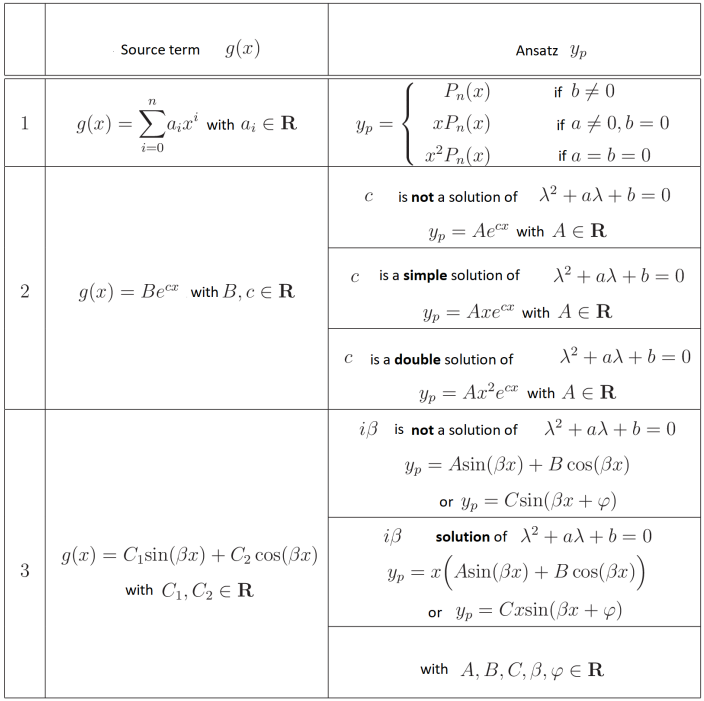
\includegraphics[width=\linewidth]{Pics/2.7.png}
% \end{figure}
% lecture notes page 50!\\
\begin{table}[H]
  \centering
  \scriptsize
  \begin{tabular}{l|l}
  Source term $g(x)$    & Ansatz $y_p$\\ \hline
  $g(x) = \sum_{i=0}^2 a_i x^i$ &
  $\left \{\begin{matrix*}[l]
    P_n(x)    & \text{if}\; b \neq 0\\
    xP_n(x)   & \text{if}\; a \neq 0, b = 0\\
    x^2P_n(x) & a=b=0
  \end{matrix*}\right.$ \\ \hline
  \multirow{6}{*}{$g(x) = Be^{cx}$} & $c$ is not a solution of $\lambda^2 + a\lambda + b = 0$\\
                                    & $y_p = Ae^{cx}$    \\ \cline{2-2}
                                    & $c$ is a simple solution of $\lambda^2 + a\lambda + b = 0$\\
                                    & $y_p = Axe^{cx}$   \\ \cline{2-2}
                                    & $c$ is a double solution of $\lambda^2 + a\lambda + b = 0$\\
                                    & $y_p = Ax^2e^{cx}$ \\ \hline
  \multirow{6}{*}{$g(x) = C_1 \text{sin}(\beta x) + C_2 \text{cos}(\beta x)$}
                        & $i\beta$ is not a solution of $\lambda^2 + a\lambda + b = 0$\\
                        & $y_p = A\;\text{sin}(\beta x) + B\;\text{cos}(\beta x)$ or \\
                        & $y_p = Cx\;\text{sin}(\beta x + \varphi)$ \\ \cline{2-2}
                        & $i\beta$ is a solution of $\lambda^2 + a\lambda + b = 0$\\
                        & $y_p = x\left(A\;\text{sin}(\beta x) + B\;\text{cos}(\beta x)\right)$ or \\
                        & $y_p = Cx\;\text{sin}(\beta x + \varphi)$
  \end{tabular}
\end{table}

\textbf{Calculator-Example: Finding roots of Polynomial}\\
The roots of a characteristic polynomial can be found with the calculater command \texttt{cPolyRoots()}.\\
Example: We want to find the roots of the following ODE:
\begin{equation}
  y''+2y'+2y = 0
\end{equation}
The characteristic polynomial is
\begin{equation}
  P(\lambda) = \lambda^2 + 2\lambda + 2
\end{equation}
Using the command $\texttt{cPolyRoots(y}^2 \texttt{+2y+2, y)}$ returns a list with the roots of the characteristic polynomial
$\texttt{\{-1-\textbf{i}, -1+\textbf{i}\}} $.
